\let\negmedspace\undefined
\let\negthickspace\undefined
\documentclass[journal]{IEEEtran}
\usepackage[a5paper, margin=10mm, onecolumn]{geometry}
%\usepackage{lmodern} % Ensure lmodern is loaded for pdflatex
\usepackage{tfrupee} % Include tfrupee package

\setlength{\headheight}{1cm} % Set the height of the header box
\setlength{\headsep}{0mm}     % Set the distance between the header box and the top of the text

\usepackage{gvv-book}
\usepackage{gvv}
\usepackage{cite}
\usepackage{amsmath,amssymb,amsfonts,amsthm}
\usepackage{algorithmic}
\usepackage{graphicx}
\usepackage{textcomp}
\usepackage{xcolor}
\usepackage{txfonts}
\usepackage{listings}
\usepackage{enumitem}
\usepackage{mathtools}
\usepackage{gensymb}
\usepackage{comment}
\usepackage[breaklinks=true]{hyperref}
\usepackage{tkz-euclide} 
\usepackage{listings}
% \usepackage{gvv}                                        
\def\inputGnumericTable{}                                 
\usepackage[latin1]{inputenc}                                
\usepackage{color}                                            
\usepackage{array}                                            
\usepackage{longtable}                                       
\usepackage{calc}                                             
\usepackage{multirow} 
\usepackage{hhline}                                           
\usepackage{ifthen}                                           
\usepackage{lscape}
\usepackage{circuitikz}
\tikzstyle{block} = [rectangle, draw, fill=blue!20, 
    text width=4em, text centered, rounded corners, minimum height=3em]
\tikzstyle{sum} = [draw, fill=blue!10, circle, minimum size=1cm, node distance=1.5cm]
\tikzstyle{input} = [coordinate]
\tikzstyle{output} = [coordinate]

\begin{document}
\bibliographystyle{IEEEtran}
\vspace{3cm}

\title{MatGeo Assignment 4.4.3}
\author{AI25BTECH11007}
 \maketitle
% \newpage
% \bigskip
{\let\newpage\relax\maketitle}

\renewcommand{\thefigure}{\theenumi}
\renewcommand{\thetable}{\theenumi}
\setlength{\intextsep}{10pt} % Space between text and floats


\numberwithin{equation}{enumi}
\numberwithin{figure}{enumi}
\renewcommand{\thetable}{\theenumi}
\textbf{Question:}\\
Equation of the line passing through the origin and making $30^\circ$
, $60^\circ$, and $90^\circ$ with the $X, Y, Z$ axes respectively is.

\bigskip

\noindent
\textbf{Solution:}
The equation of a line passing through the origin and making angles 
$\alpha, \beta, \gamma$ with the $X, Y, Z$ axes respectively is given by
\[
\frac{x}{\cos \alpha} = \frac{y}{\cos \beta} = \frac{z}{\cos \gamma}.
\]

Here, $\alpha = 30^\circ, \beta = 60^\circ, \gamma = 90^\circ$.\\

Direction Cosines,
\[
\cos 30^\circ = \frac{\sqrt{3}}{2}, \quad 
\cos 60^\circ = \frac{1}{2}, \quad 
\cos 90^\circ = 0.
\]

\[
\frac{x}{\frac{\sqrt{3}}{2}} = \frac{y}{\frac{1}{2}} = \frac{z}{0}.
\]


Final equation of the line ,
\[
y = \frac{x}{\sqrt{3}}, \quad z = 0.
\]

\begin{figure}[H]
    \centering
    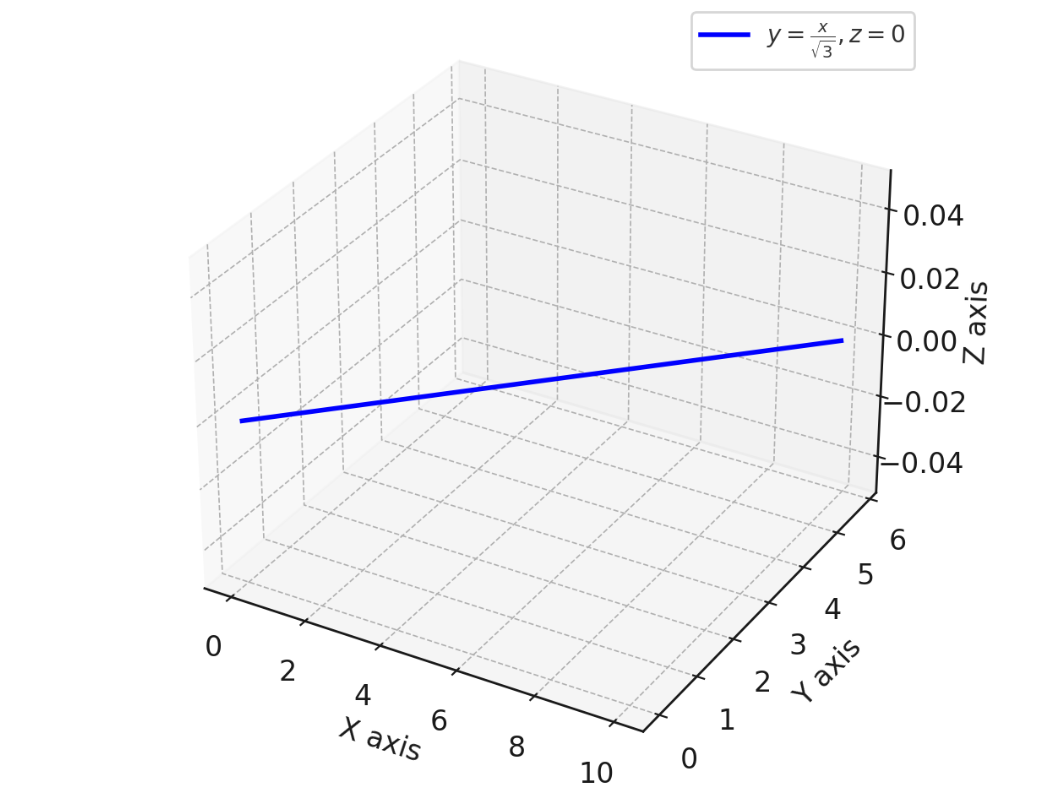
\includegraphics[width=0.85\linewidth]{figs/image.png}
    \caption{Plot}
    \label{fig:placeholder}
\end{figure}
\end{document}
